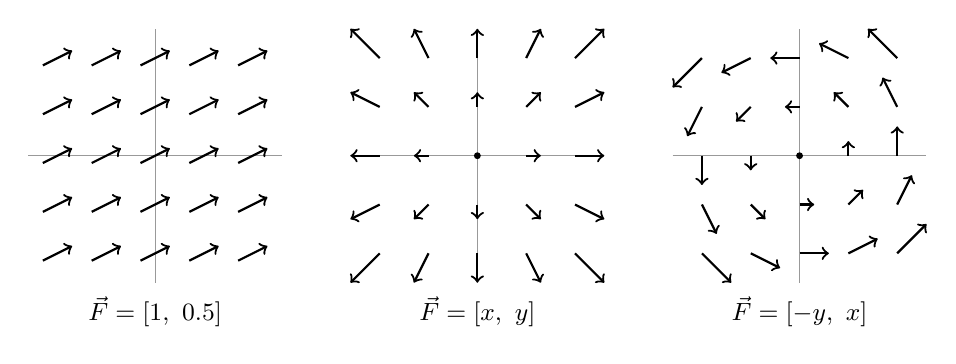
\begin{tikzpicture}[scale=0.62]
\foreach \pan/\nav/\lab in {0/a/{$\vec F = [1,\ 0.5]$}, 1/b/{$\vec F = [x,\ y]$}, 2/c/{$\vec F = [-y,\ x]$}} {
\begin{scope}[shift={(\pan*6.6,0)}]
\draw[black!40] (-2.6,0)--(2.6,0); \draw[black!40] (0,-2.6)--(0,2.6);
\node[font=\small] at (0,-3.2) {\lab};
\end{scope}}
% konstant felt
\begin{scope}[shift={(0,0)}]
\foreach \x in {-2,-1,0,1,2} \foreach \y in {-2,-1,0,1,2} \draw[->,thick] (\x-0.3,\y-0.15)--++(0.6,0.3);
\end{scope}
% radielt felt, skalert 0.3
\begin{scope}[shift={(6.6,0)}]
\foreach \x in {-2,-1,0,1,2} \foreach \y in {-2,-1,0,1,2} {
  \ifnum\x=0 \ifnum\y=0 \fill (0,0) circle (2pt); \else \draw[->,thick] (\x,\y)--++({0.3*\x},{0.3*\y}); \fi
  \else \draw[->,thick] (\x,\y)--++({0.3*\x},{0.3*\y}); \fi }
\end{scope}
% rotasjonsfelt, skalert 0.3
\begin{scope}[shift={(13.2,0)}]
\foreach \x in {-2,-1,0,1,2} \foreach \y in {-2,-1,0,1,2} {
  \ifnum\x=0 \ifnum\y=0 \fill (0,0) circle (2pt); \else \draw[->,thick] (\x,\y)--++({-0.3*\y},{0.3*\x}); \fi
  \else \draw[->,thick] (\x,\y)--++({-0.3*\y},{0.3*\x}); \fi }
\end{scope}
\end{tikzpicture}
